\documentclass[12pt, a4papre]{article}
\usepackage[catalan]{babel}
\usepackage[unicode]{hyperref}
\usepackage{amsmath}
\usepackage{amssymb}
\usepackage{amsthm}
\usepackage{xifthen}
\usepackage{listings}
\usepackage{float}
\usepackage{siunitx}
\usepackage{graphicx}
\usepackage{indentfirst}

\newcommand{\norm}[1]{\lvert #1 \rvert}
\graphicspath{ {./Images/} }

\hypersetup{
    colorlinks = true,
    linkcolor = blue
}

\author{Elexioma de l'acció}
\title{P109 Rosant el pal}
\date{}

\begin{document}
	\maketitle
	
	
	\begin{proof} Veiem primer el cas de $\mathbb{R}^2$. El minim nombre de rectes que es necessiten al començar per a poder cubrir tot $\mathbb{R}^2$ es 4. Si tinguessim punts suficients com per a traçar nomes 3 rectes aleshores cualsevols grups de 4 punts pertenyents a les rectes en tindrà com a minim 2 pertenyents a una recta ja existent, i per tant la unica recta que es podria formar amb aquests punts es la que ja existeix. La forma optima de crear 4 rectes a partir de punts usa nomes 10 punts, ja que com ha minim ha de usar $4\cdot4 - {4\choose 2}$ punts. La construcció es fa a base de posar al pla 4 rectes encreuades dos a dos sense que intersequin 3 al mateix punt i posar els punts a les 6 interseccions, també cal posar un punt extra a cada recta per a que puguin ser creades ja que d'interseccions una recta en te nomes 3 i es necessiten 4 punts per a crearla. 
	
	Un cop tenim les 4 rectes, qualsevol punt podrà ser pintat per una recta que passa per el punt i no es paralela a cap de les originals, ja que per força les creuarà totes.
	
	Un cop tenim el cas de $\mathbb{R}^2$ veiem que el cas de $\mathbb{R}^3$ es molt semblant. El nombre mínim de plans que es necessiten al començar per a cubrir tot $\mathbb{R}^3$ es 4. Si tinguessim punts suficients per a traçar nomes 3 plans aleshores per la mateixa rao del cas de $\mathbb{R}^2$ no es podria pintar cap punt que no estigues contingut dins dels 3 plans. El minim nombre de punts per a fer tres plans usa una construcció que aprofita la de $\mathbb{R}^2$. 
	
	Justifiquem primer que amb si es poden crear 4 plans no paralels i que no sintersequen 2 a 2 en una mateixa recta aleshores això sha de fer en com a minim 20 punts. El primer plà per la justificació anterior sha de fer en com a minim 10 punts. El segon plà podem aprofitar 4 punts del primer pero si usessim més hauria de estar inclos dins del pla i seria paralel, per tant en faltarien 6 per a completar els 10 necessaris. El tercer plà podem usar 4 del primer i 4 del segon, pero un d'ells estara a la intersecció aixi que haurem de completar amb 3. Finalment el ultim podem usar 4 del primer 4 del segon i 4 del tercer, pero d'aquests 3 estaran en interseccions aixi que haurem d'afegir un. Per tant com a minim s'haurà de fer amb 20 punts. Es a dir que com a minim necessita $4\cdot10 punts -  2{4\choose 3} - 2 {4\choose 2}$ punts
	
	Veiem ara una construccio dels 4 plans amb 20 punts.
	
	\begin{itemize}
		\item Creem el primer pla amb 10 punts de la mateixa forma que a $\mathbb{R}^2$. 
		\item El segon plà usem els 4 punts que s'han usat per a crear una recta original del primer pla i hi afegim 6 més, 3 que seran intersecció 2 a 2 de rectes que surten dels punts creats i no estaran continguts dins del primer plà i 3 mes per a poder definir la recta a partir dels 3 alineats. 
		\item El tercer pla el podem crear a partir de una segona recta del primer plà i tres punts alineats a un dels punts de la recta agafada pertanyents al 2n pla, que existeixen per construcció. Ara simplement considerant un dels punts del pla 1 que no pertanyi a 2, aixecarem amb 2 nous punts una recta paral·lela a una de les noves creades el pla 2. Amb un tercer punt unirem tres punts consecutius per a crear la recta necessaria per a crear el pla.
	
		\item El quart plà usarà uns altres 4 punts del primer plà (diferents als usats pel 2n plà) i també usarà 3 punts mes del 2n pla que estiguin alineats (diferents a tots 4 que hem agafat). A partir d'aquests 7 punts, nomes afegint 3 ja podrem formar un pla que no serà paral·lel a cap dels 2. Finalment afegint un sol punt podrem crear un quart plà, ja que podem tornar a agafar 4 del primer pla, de les cuals 2 han de formar part del pla 2 i pla 3 respectivament. Agafem tambe les 3 que estan al pla 2 i al pla 3, per tant tenim 9 punts. Amb un mes ja podem formar pla, afegint un ultim punt a tres punts consecutirs d'aquests 9 que es poden conseguir amb la construcció pertinent.
		
		 
	\end{itemize}
	
	Per tant amb nomes 20 punts, es podrà arribar a qualsevol punt de $\mathbb{R}^3$ si seguim la mateixa estrategia que amb  $\mathbb{R}^2$, es a dir, a partir del punt traçar una recta no paralela a cap dels plans.
	
	\begin{figure}[H]
		\begin{center}
		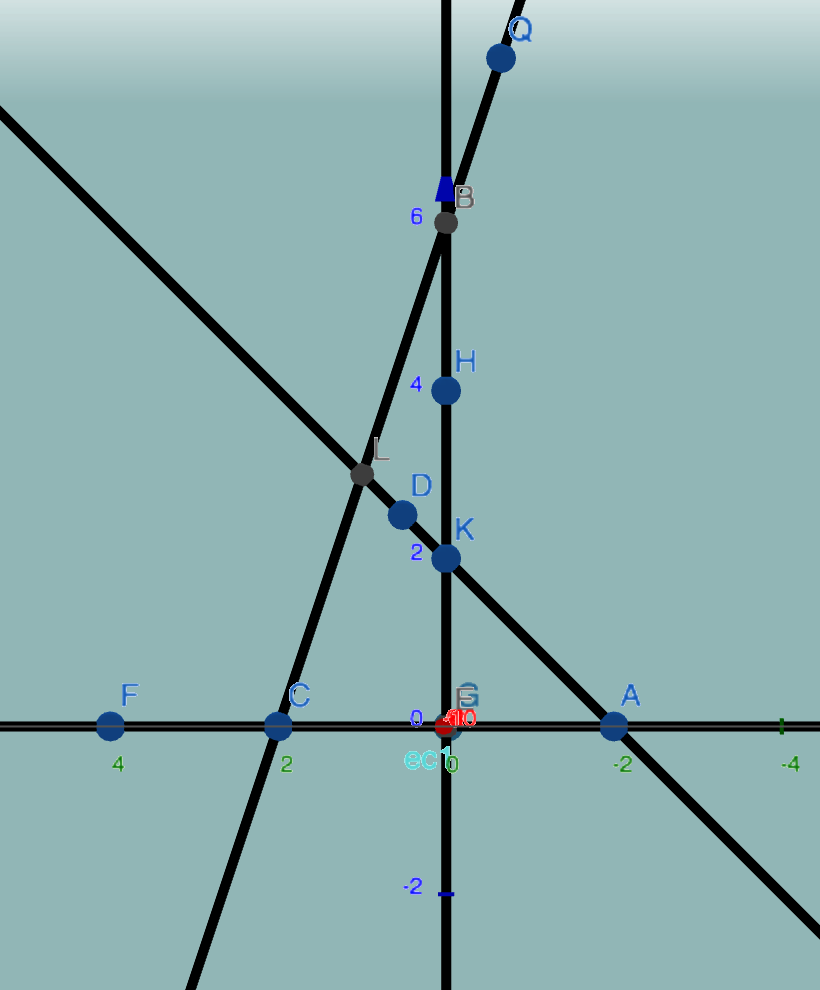
\includegraphics[width=60mm]{primer_pla.png}
		\caption{Primer pla}
		\end{center}
	\end{figure}
	
	\begin{figure}[H]
		\begin{center}
		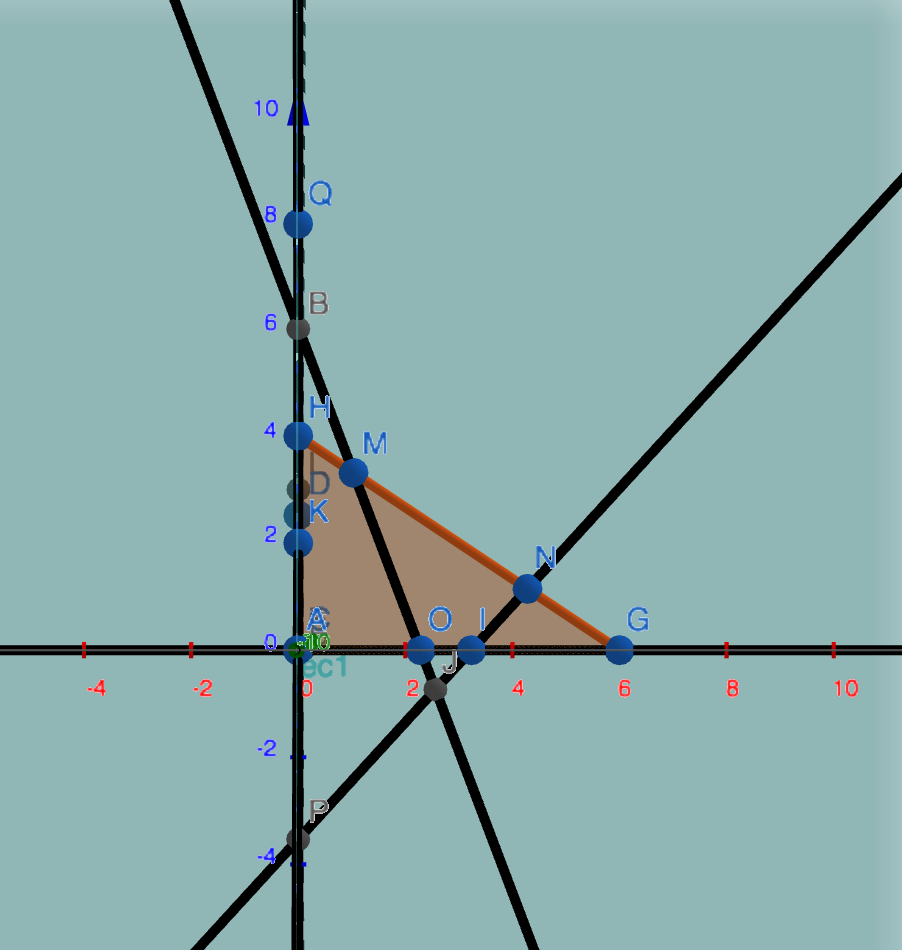
\includegraphics[width=60mm]{segon_pla.png}
		\caption{Segon pla}
		\end{center}
	\end{figure}
	
	\begin{figure}[H]
		\begin{center}
		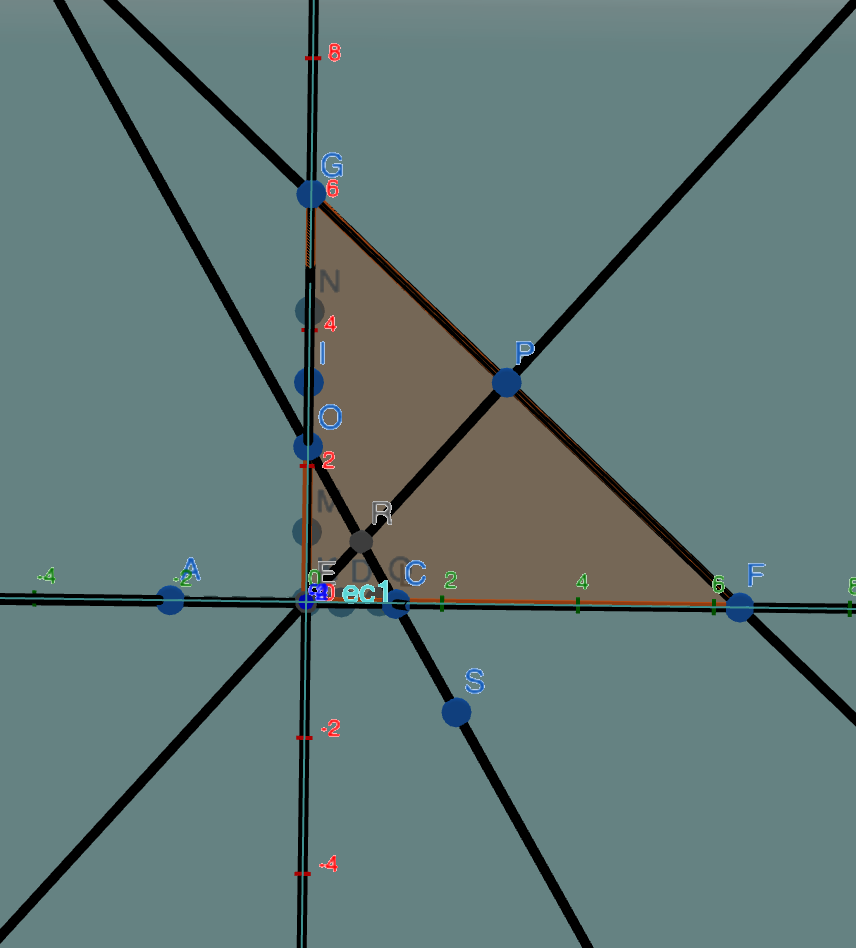
\includegraphics[width=45mm]{tercer_pla.png}
		\caption{Tercer pla}
		\end{center}
	\end{figure}
	
	\begin{figure}[H]
		\begin{center}
		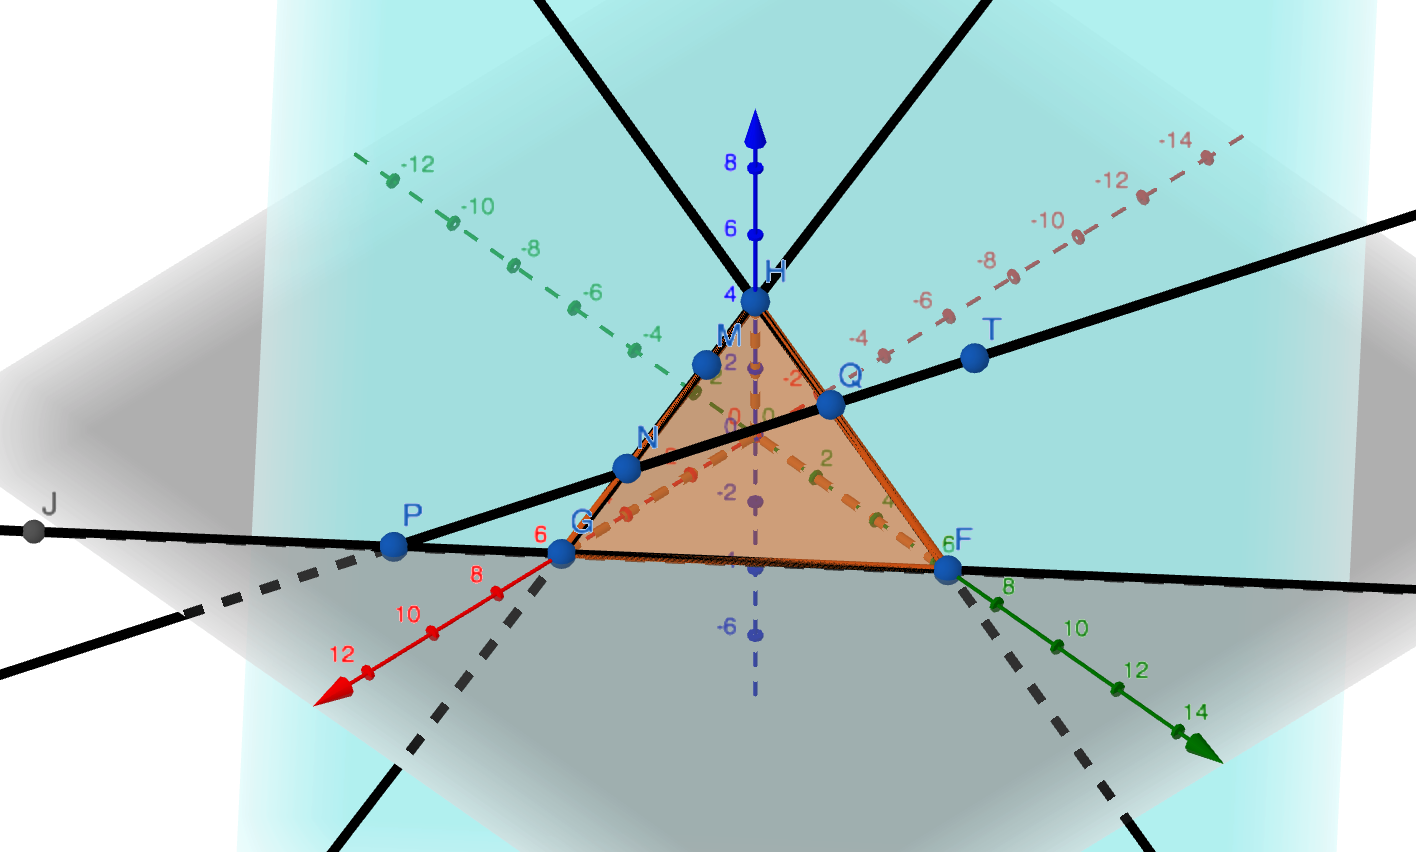
\includegraphics[width=60mm]{quart_pla.png}
		\caption{Quart pla}
		\end{center}
	\end{figure}
	
	\begin{figure}[H]
		\begin{center}
		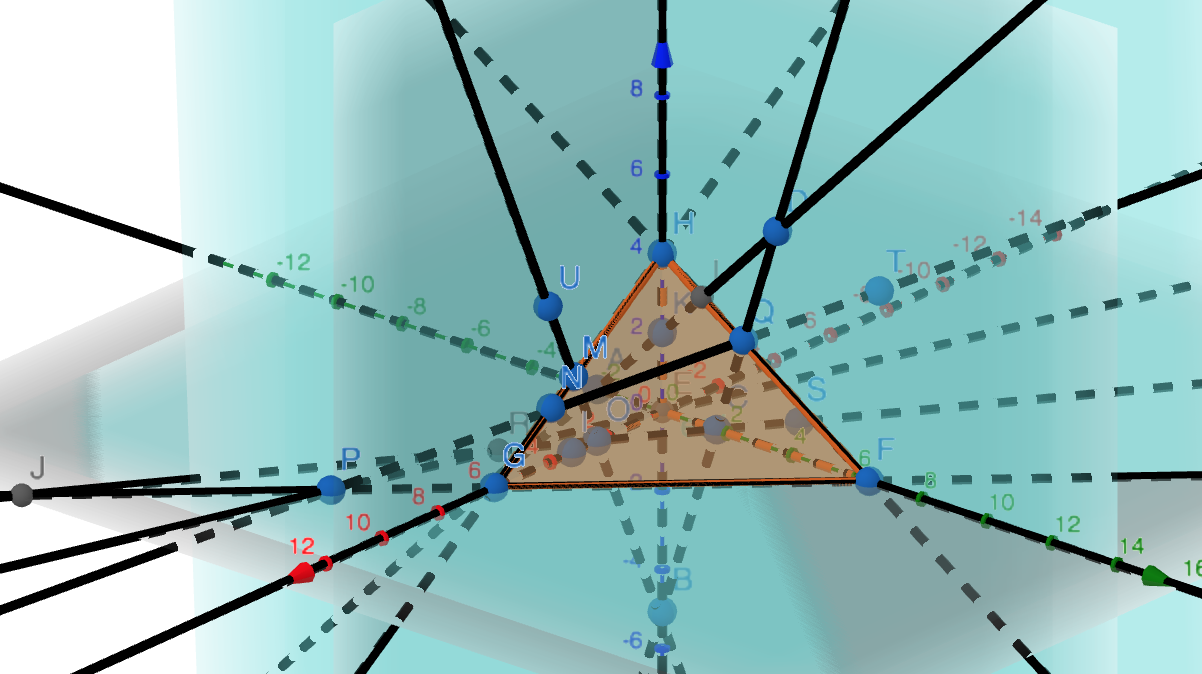
\includegraphics[width=60mm]{final.png}
		\caption{Resultat final}
		\end{center}
	\end{figure}
	
	\end{proof}
	
	
	
	
\end{document}